\section{Introduction to Physical Oceanography: Geophysical Fluid
Dynamics}\label{introduction-to-physical-oceanography-geophysical-fluid-dynamics}

\subsection{Course text:}\label{course-text}

Much of the course material is based on the textbook ``Introduction to
Geophysical Fluid Dynamics'\,' by Benoit Cushman-Roisin and Jean-Marie
Beckers, 2011, Academic Press. The book is available online through the
library.

\subsection{Why Geophysical Fluid
Dynamics?}\label{why-geophysical-fluid-dynamics}

\begin{itemize}
\tightlist
\item
  What is it:?

  \begin{itemize}
  \tightlist
  \item
    The study of the motion of fluids in the atmosphere and oceans, with
    a focus on large-scale phenomena.
  \end{itemize}
\item
  Why is it important?

  \begin{itemize}
  \tightlist
  \item
    Applications:
    \begin{itemize}
    \tightlist
    \item
      Weather forecasting
    \item
      Climate modeling
    \item
      Ocean circulation studies
    \item
      Environmental monitoring
    \end{itemize}
  \item
    Slides:

    \begin{itemize}
    \tightlist
    \item
      Hurricane
    \item
      North Pacific Gyre

      \begin{itemize}
      \tightlist
      \item
        have velocity on here!
      \end{itemize}
    \item
      Overturning Circulation

      \begin{itemize}
      \tightlist
      \item
        strength of circulation is about 10 Sv (1 Sv = 10\^{}6 m\^{}3/s)
      \end{itemize}
    \end{itemize}
  \end{itemize}
\end{itemize}

\subsection{Characteristics:}\label{characteristics}

\begin{itemize}
\tightlist
\item
  Normal fluid dynamics:

  \begin{itemize}
  \tightlist
  \item
    pressure moves water
  \item
    water can exert \emph{shear stresses} on itself.
  \end{itemize}
\item
  Plus:

  \begin{itemize}
  \tightlist
  \item
    Earth's rotation matters
  \item
    Density stratification matters
  \end{itemize}
\item
  Scales:

  \begin{itemize}
  \tightlist
  \item
    Hurricane:

    \begin{itemize}
    \tightlist
    \item
      \(L = 800\) km across, \(U = 55\) m/s winds
    \item
      translation speed \(c= 250 km/ d = 3 m/s\)
    \item
      timescale?

      \begin{itemize}
      \tightlist
      \item
        rotation = \(\pi 400\times10^3 / 55 = 8 h\);
      \item
        translation = \(800 /250 = 3.2 d\);
      \end{itemize}
    \end{itemize}
  \item
    North Pacific Gyre:

    \begin{itemize}
    \tightlist
    \item
      \(L = 10_000\) km across, \(U = 1\) m/s\$ (in Kurosio, much slower
      elsewhere)
    \item
      timescale: \textgreater{} 100 d in Kuroshio.
    \end{itemize}
  \item
    Overturning Circulation:

    \begin{itemize}
    \tightlist
    \item
      \(H = 4000 m\),
    \item
      \(w = <0.01 m/d = 3 m /y = 10^{-7} \mathrm{m/s}\) (how do we
      measure this?, can we?)

      \begin{itemize}
      \tightlist
      \item
        \(10^{7} m^3/s / 10^7 m / 10^7 m = 10^{-7} \mathrm{m/s}\).
      \end{itemize}
    \item
      timescale is about 1000 years.
    \end{itemize}
  \item
    Rotation timescale:

    \begin{itemize}
    \tightlist
    \item
      \(\Omega = \frac{2\pi}{24 \times 3600} \approx 7.27 \times 10^{-5} \mathrm{rad/s}\).
    \item
      \(f = 2\Omega \sin(\phi)\), where \(\phi\) is latitude.
    \item
      \(f=0\) at equator, \(\pm2\Omega\) at poles, and
      \(\pm10^{-4} \mathrm{rad/s}\) at 45 N/S.
    \item
      So at the equator, the \emph{inertial period} tends to infinity!.
      At 45 N it is 17.45 h. At the north pole it is 12 h.
    \item
      motions that last longer than the inertial period are called
      \emph{geostrophic}.
    \end{itemize}
  \item
    Aspect ratio:

    \begin{itemize}
    \tightlist
    \item
      very flat! 10000 km/4 km = 1:2500.
    \item
      horizontal velocities are much larger than vertical ones.
      \(U \ sim 0.01 m/s\) versus \(W \sim 10^{-7} m/s\). (\(1:10^5\)
      instead of \(1:2.5\times10^3\)).
    \end{itemize}
  \end{itemize}
\item
  Slide:

  \begin{itemize}
  \tightlist
  \item
    Table 1.2 and Figure 1.7 from CR.
  \end{itemize}
\end{itemize}

\subsection{Course structure:}\label{course-structure}

\begin{itemize}
\tightlist
\item
  Discussion of the course structure, assignments, and expectations.
\end{itemize}

\section{Thermodynamics of water}\label{thermodynamics-of-water}

\begin{itemize}
\tightlist
\item
  T: energy of water due to molecular vibrations.
\item
  Salt: g solids/ kg water.

  \begin{itemize}
  \tightlist
  \item
    ratios of constituent solids relatively constant in the ocean

    \begin{itemize}
    \tightlist
    \item
      residence time of a salt solids is on order of 10\^{}6 years or so
      (versus 1000 y for mixing timescale), so well-mixed except very
      close to a river.
    \item
      Some small geographical differences (TEOS10 is a good resource).
    \end{itemize}
  \item
    about 35 g/kg;

    \begin{itemize}
    \tightlist
    \item
      measured via deriving the mass of solids
    \item
      titrate with silver nitrate to precipitate chloride, then measure
      the mass of the precipitate.
    \item
      measure via conductivity

      \begin{itemize}
      \tightlist
      \item
        fast and electronic, therefore easier.
      \item
        depends on temperature and pressure as well, so need corrections
        to get salinity
      \end{itemize}
    \end{itemize}
  \end{itemize}
\item
  Pressure:

  \begin{itemize}
  \tightlist
  \item
    force that molecules exert on one another due to their kinetic
    energy.
  \item
    omni-directional
  \item
    \(\delta\mathbf{F} = P \delta\mathbf{A}\)
  \item
    \(N / m^2 = Pa\)
  \item
    A decibar is defined as \(\mathrm{dbar}\) = 10\^{}4 Pa approx weight
    of 1 m of water
  \end{itemize}
\item
  Density:

  \begin{itemize}
  \tightlist
  \item
    mass per unit volume
    (\(\rho_0(S=0\ \mathrm{psu}, T=4\ \mathrm{°C} , P=1\ \mathrm{atm}) = 1000\ \mathrm{kg\,m^{-3}}\)).
  \item
    Equation of state is very non-linear: \[\rho = \rho(S, T, P)\]

    \begin{itemize}
    \tightlist
    \item
      \(S\) is salinity, \(T\) is temperature, and \(P\) is pressure.
    \item
      evaluated on a computer via polynomial fits. Historically PSS-78,
      now TEOS10, though we will use PSS-78 mostly for convenience.
    \item
      SLIDE OF EOS.
    \item
      Thermal expansion coefficient
      \(\alpha = -\frac{1}{\rho}\frac{\partial \rho}{\partial T}\),
      haline contraction:
      \(\beta = \frac{1}{\rho}\frac{\partial \rho}{\partial P}\).
    \item
      \(\alpha\) is about \(2\times10^{-4} \mathrm{K}^{-1}\) at
      \(S=35\ \mathrm{psu}, T=15\ \mathrm{°C}, P=1\ \mathrm{atm}\).

      \begin{itemize}
      \tightlist
      \item
        So for a 1 K change in temperature, the density changes by about
        0.2 kg/m\^{}3.
      \end{itemize}
    \item
      \(\beta(35, 15, 0)\) is about
      \(7.5 \times 10^{-4} \mathrm{psu}^{-1}\).

      \begin{itemize}
      \tightlist
      \item
        So for a 1 psu change in salinity, the density changes by about
        0.7 kg/m\^{}3.
      \end{itemize}
    \item
      \(\gamma(35, 15, 0)\) is about
      \(4.5 \times 10^{-6} \mathrm{dbar}^{-1}\).

      \begin{itemize}
      \tightlist
      \item
        So for a 1 dbar change in pressure, the density changes by about
        .0045 kg/m\^{}3.
      \item
        Over 4000 dbar depth of ocean
        \(\delta \rho \approx 18 \mathrm{kg/m^3}\).
      \end{itemize}
    \end{itemize}
  \item
    Bousinesque Approximation:

    \begin{itemize}
    \tightlist
    \item
      small variations in density can be ignored except in ``buoyancy''
      terms (where \(\rho\) is multiplied by gravity).
    \item
      eg \(\rho \approx \rho_0 + \delta\rho\), where \(\delta\rho\) is
      small.
    \item
      this particularly comes up in the momentum equations, where we
      ignore the density variations compared to the velocity variations:
      momentum (per \(m^3\)) is \(\rho u \approx \rho_0 u\), so terms
      like
      \(\partial (\rho u)/\partial x \approx \rho_0 \partial u/\partial x\).
    \item
      \(\delta\rho/\rho_0 \approx 0.04\) over the whole ocean, and much
      less in the horizontal

      \begin{itemize}
      \tightlist
      \item
        eg the density of fresh water is \(1000\ \mathrm{kg/m^3}\)
        whereas the density of seawater at 35 psu and 15 deg C is
        \(1026\ \mathrm{kg/m^3}\).
      \end{itemize}
    \end{itemize}
  \item
    Potential Temperature and Density

    \begin{itemize}
    \tightlist
    \item
      Salinity doesn't change due to compression by the weight of
      sewater above, but temperature and density go up without changing
      the total energy of the water (adiabatic temperature increase)
    \item
      Temperature and salinity largely set at the ocean surface, and
      following a parcel of water only change at depth due to mixing or
      compression.
    \item
      We often remove the compressive effect so on both temperature and
      density to better understand where the water came from and what
      mixing it has undergone.
    \item
      Potential temperature \(\theta\) is the temperature of a parcel of
      water if it were brought back to the surface with no heat exchange
      with the water around it.

      \begin{itemize}
      \tightlist
      \item
        slide of deep T cast and potential temperature.
      \item
        slide with section of the two
      \end{itemize}
    \item
      Potential density \(\sigma\) is the density of a parcel of water
      if it were brought back to the surface with no heat exchange with
      the water around it.

      \begin{itemize}
      \tightlist
      \item
        \(\sigma_{\theta} = \rho(S, \theta, 0) - 1000\ \mathrm{kg/m^3}\).
      \item
        \(\sigma_{\theta}\) is often used instead of \(\rho\) in
        oceanography.
      \item
        note that the potential density is more nonlinear than potential
        temperature, and sometimes it is referenced to other depths than
        the surface.
      \item
        show slide of potential densities.
      \end{itemize}
    \end{itemize}
  \end{itemize}
\end{itemize}

\section{Conservation of a tracer (fluid dynamics
``review'')}\label{conservation-of-a-tracer-fluid-dynamics-review}

Consider a tracer with a concentration \(C(x,y,z,t)\) (with units like
\(\mathrm{g/m^3}\)) that is advected by a flow with velocities
\(\mathbf{u} = (u,v,w)\), where \(u\) is the velocity in the \(x\)
direction, \(v\) in the \(y\) direction, and \(w\) in the \(z\)
direction.

Now consider a volume \(V = \delta x \delta y \delta z\) that is a fixed
cube in space. The rate of change of tracer in the volume is given by
the sum of \emph{transport} of tracers across the six faces into the
volume:

\[ \int_V \frac{\partial C}{\partial t}  \, dV = -\int_S \mathbf{F_C} \cdot \mathbf{n} \, dS\]

where \(\mathbf{F_C}\) is the \emph{flux} of \(C\), \(S\) is the surface
of the volume and \(\mathbf{n}\) is the outward normal vector to the
surface. Note that the \emph{transport} has units like g/s, and the
\emph{flux} \(F_C\) has units like g/m\^{}2/s.

There are two types of fluxes that can change \(C\), the \emph{advective
flux} and the \emph{diffusive flux}. The \emph{advective flux} is that
due to the flow of the water carrying the tracer and is given by
\[\mathbf{F_C} = C \mathbf{u}\] Supposing for a second that diffusive
fluxes are negligible, we can write the equation as

\[ \int_V \frac{\partial C}{\partial t}  \, dV = -\int_S C \mathbf{u} \cdot \mathbf{n} \, dS\]

We can evaluate these terms on our hypothetical volume \(V\):
\pandocbounded{\includesvg[keepaspectratio]{./imgs/S01_cube.svg}} so
\[\delta x \delta y \delta z \frac{\partial C}{\partial t} = - (C(x+\delta x,y,z) u(x+\delta x, y, z) - C(x,y,z) u(x, y, z))\delta y\, \delta z - (C(x, y+\delta y,z) v(x, y+\delta y, z) - C(x,y,z) v(x, y, z))\delta x\, \delta z - (C(x, y, z +\delta z) w(x, y, z+\delta z) - C(x,y,z) w(x, y, z))\delta x\, \delta y \]

or simplifying:

\[\frac{\partial C}{\partial t} = - \left( \frac{C(x+\delta x,y,z) u(x+\delta x, y, z) - C(x,y,z) u(x, y, z)}{\delta x} + \frac{C(x, y+\delta y,z) v(x, y+\delta y, z) - C(x,y,z) v(x, y, z)}{\delta y} + \frac{C(x, y, z +\delta z) w(x, y, z+\delta z) - C(x,y,z) w(x, y, z)}{\delta z} \right)\]

or as the volume becomes infinitesimally small:

\[\frac{\partial C}{\partial t} = - \left( \frac{ \partial}{\partial x} \left(uC\right) + \frac{\partial}{\partial y}\left(vC\right) + \frac{\partial}{\partial z}\left(wC\right) \right) + \mathrm{diffusion}\]
or
\[\frac{\partial C}{\partial t} = - \nabla \cdot \left(\mathbf{u}C\right) + \mathrm{diffusion}\]

This equation is the \emph{advection equation} and, again,
\(\mathbf{u}C\) is the \emph{advective flux} of the tracer \(C\).

Note we could also have done:
\[ \int_V \frac{\partial C}{\partial t}  \, dV = -\int_S C \mathbf{u} \cdot \mathbf{n} \, dS\]
and by Gauss's theorem, we can convert the surface integral to a volume
integral:
\[\int_V \frac{\partial C}{\partial t}  \, dV = -\int_V \nabla \cdot \left(C \mathbf{u} \right) \, dV\]

which gives the same equation as above.

\subsection{Diffusive fluxes}\label{diffusive-fluxes}

Diffusive fluxes are those due to the random motion of the tracer
molecules, and are given by Fick's law: \[\mathbf{F_C} = -K \nabla C\]

where \(K\) is the diffusivity of the tracer (with units like m\^{}2/s).
The diffusivity is a measure of how fast the tracer spreads out in
space. For example, for temperature,
\(K \approx 10^{-7} \mathrm{m^2/s}\), and for salt,
\(K \approx 10^{-9} \mathrm{m^2/s}\). Substituting this into the
conservation equation gives:
\[\frac{\partial C}{\partial t} = - \nabla \cdot \left(\mathbf{u}C\right) + K \nabla^2 C\]
This is the \emph{advection-diffusion equation} for a tracer \(C\).

\begin{itemize}
\tightlist
\item
  All mixing takes place at the molecular level, but the diffusivity
  co-efficient is very small.

  \begin{itemize}
  \tightlist
  \item
    tends to act on small-scales
  \item
    turbulent \emph{stirring} can enhance the fluxes, and is often
    parameterized as an ``eddy diffusivity'' or ``turbulent
    diffusivity'' \(K_T\),
  \item
    \(K_T\) is much larger than molecular, but acts on larger scales.
  \end{itemize}
\end{itemize}

\subsection{Conservation of water
mass}\label{conservation-of-water-mass}

The conservation of water mass can be written:
\[\frac{\partial \rho}{\partial t} + \nabla \cdot (\rho \mathbf{u}) = \mathrm{diffusion}\]
Ignoring diffusion, we can re-write as:
\[\frac{1}{\rho} \left(\frac{\partial \rho}{\partial t} +\mathbf{u}\cdot\nabla\rho\right) = - \nabla \cdot \mathbf{u}\]
- density of seawater only changes by 3\% or so in the ocean, so the
left hand side is small, or
\[\frac{\partial \rho}{\partial t} +\mathbf{u}\cdot\nabla\rho \approx 0\]
- so the right hand side is also small, or
\(\nabla \cdot \mathbf{u} \approx 0\). - this is called the
\emph{incompressibility approximation} and is a very good approximation
for the ocean. - it is much less good for the atmosphere, but sometimes
gets used there as well if flows are not too vertical. - The integral
form of this is: - \[ \int_S \mathbf{u} \cdot \mathbf{n} \, dS = 0\] -
or the net flow of water into a volume is zero.

\subsection{Eulerian vs Lagrangian reference
frames:}\label{eulerian-vs-lagrangian-reference-frames}

Physical laws are defined following a parcel of water (Lagrangian) For
the above, the physical law is that the change of tracer following the
fluid is due to diffusion: \[\frac{D C}{D t} = K\nabla^2 C\] From the
above, we see that if the flow is incompressible, then
\[\frac{D \rho}{D t} = \frac{\partial \rho}{\partial t} + \mathbf{u}\cdot\nabla\rho = 0\]
\(\frac{D C}{D t}\) is the \emph{material derivative} of \(C\), and is
the change of \(C\) following a parcel of water. It is also called the
\emph{Lagrangian derivative}.

The laws above were derived fixed in space, and so we derived an
equation for the \emph{Eulerian derivative} of \(C\):
\[\frac{\partial C}{\partial t} + \mathbf{u}\cdot\nabla C = K\nabla^2 C\]

As an example, consider a stream flowing at speed \(U\) in the \(x\)
direction, and suppose the tracer is high upstream and low downstream.
Ignoring diffusion, if we follow the stream at a speed \(U\), then the
tracer will not change. If we are sitting stationary on the bank, then
\(\partial C/\partial t = -U\partial C/\partial x\), which will be
positive because \(dC/dx < 0\) (the tracer is high upstream and low
downstream).

\begin{figure}
\centering
\pandocbounded{\includesvg[keepaspectratio]{./imgs/S01_river.svg}}
\caption{Eulerian vs Lagrangian}
\end{figure}

\section{Conservation of momentum}\label{conservation-of-momentum}

The conservation of momentum is given by Newton's second law:
\[\frac{D}{Dt}\int_V \rho \mathbf{u} \, \mathrm{d}V = \sum \mathbf{F}\]
- what are the forces? - pressure gradient forces - viscous stress
forces - Coriolis force - gravity force - The first two are interfacial
forces that act on the edges of a given fluid volume. - The last two are
body forces that act on the whole volume.

\subsection{gravity force:}\label{gravity-force}

Pretty straight forward, and only acts in the ``vertical'' direction: -
\(\rho \delta V \frac{D\mathbf{u}}{Dt} = -\rho \delta V g \mathbf{k} + ...\)
- \(\mathbf{k}\) is the unit vector in the vertical direction, and \(g\)
is the acceleration due to gravity. - or \(\frac{Dw}{Dt} = -g + ...\)

\subsection{Pressure gradient force:}\label{pressure-gradient-force}

The pressure gradient force is a huge part of what gives fluids a very
different class of behaviour than solids. If water piles up somewhere,
it creates pressure gradients inside the fluid that can drive
accelerations. Note this is not just the piled up water pouring downhill
- the pressure gradient is felt throughout the water column, so even
deep water will move. - a demo using a small tank is very nice here,
with a dye streak to show that all the water moves, not just the surface
when there is a wave in the tank.

To derive the pressure gradient force we can consider a small cube
again:

\begin{figure}
\centering
\pandocbounded{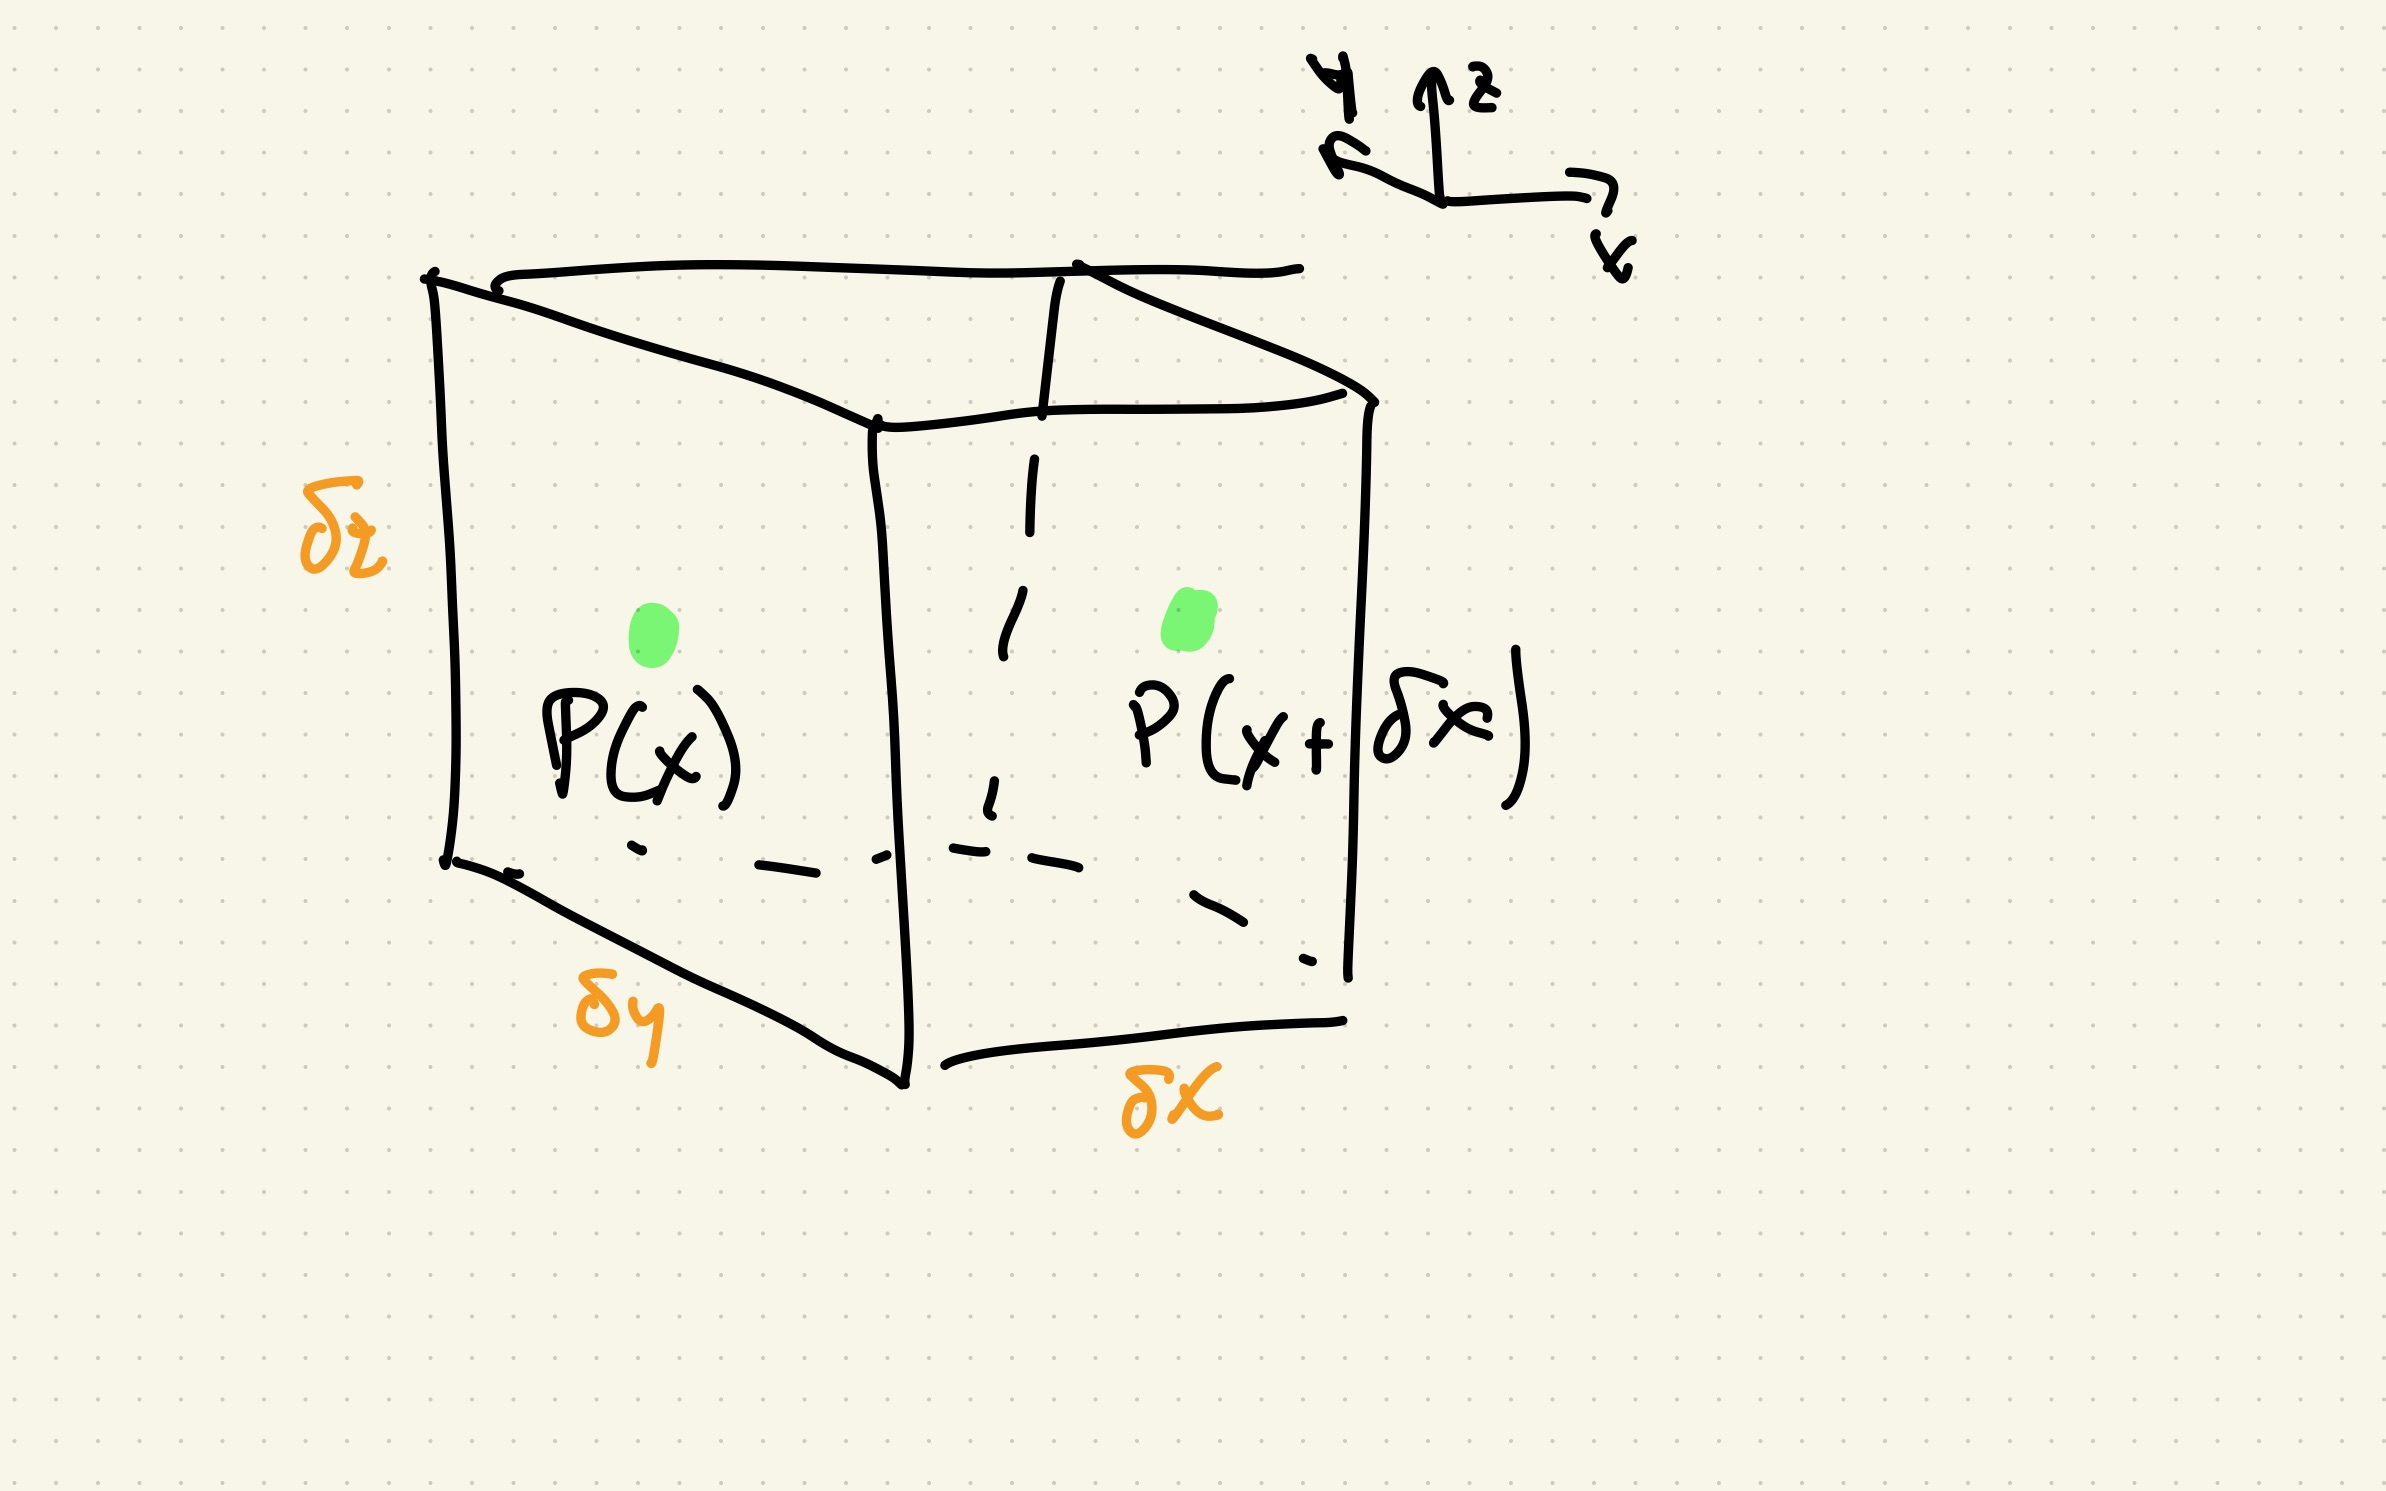
\includegraphics[keepaspectratio]{./imgs/S01_pgfcube.jpg}}
\caption{Derivation of pressure gradient force}
\end{figure}

\begin{itemize}
\tightlist
\item
  Let's just consider the forces in the x-direction; these are exerted
  on the two faces perpendicular to the x-axis:

  \begin{itemize}
  \tightlist
  \item
    \[\rho \delta x\, \delta y, \delta z \frac{D u}{Dt} = -\left(P(x+\delta x,y,z) - P(x,y,z)\right) \delta y \delta z\]
  \item
    or
  \item
    \[\frac{D u}{Dt} = -\frac{1}{\rho}\left(\frac{\partial P}{\partial x}\right)+ ...\]
  \item
    the same applies in the y- and z-directions, so we can write the
    momentum equation as:
  \item
    \[\frac{D \mathbf{u}}{Dt} = -\frac{1}{\rho}\nabla P -g\mathbf{k} + ...\]
  \end{itemize}
\end{itemize}

\subsubsection{Estimating pressure: hydrostatic
approximation}\label{estimating-pressure-hydrostatic-approximation}

In general in fluid dynamics, pressure can be ``dynamic'' and due to the
motion of the fluid. However, if vertical accelerations are small
compared to the acceleration due to gravity, then we can assume that the
pressure is hydrostatic:
\[ \frac{1}{\rho}\frac{\partial P}{\partial z} = - g - \frac{Dw}{Dt} \approx -g\]
if \(|Dw/Dt| \ll g\). - except for surface waves, and vigorous
convection, this approximation is very good in the ocean, and therefore
we can calculate the pressure at a depth \(z\) if we know the density
and the seasurface height \(\eta\)
\[ P(z) = P(\eta) + \int_z^{\eta} \rho g \, dz'\] where \(P(\eta)\) is
the sealevel pressure (usually near 10 dbar or 10\^{}5 Pa) at the ocean
surface.

\begin{figure}
\centering
\pandocbounded{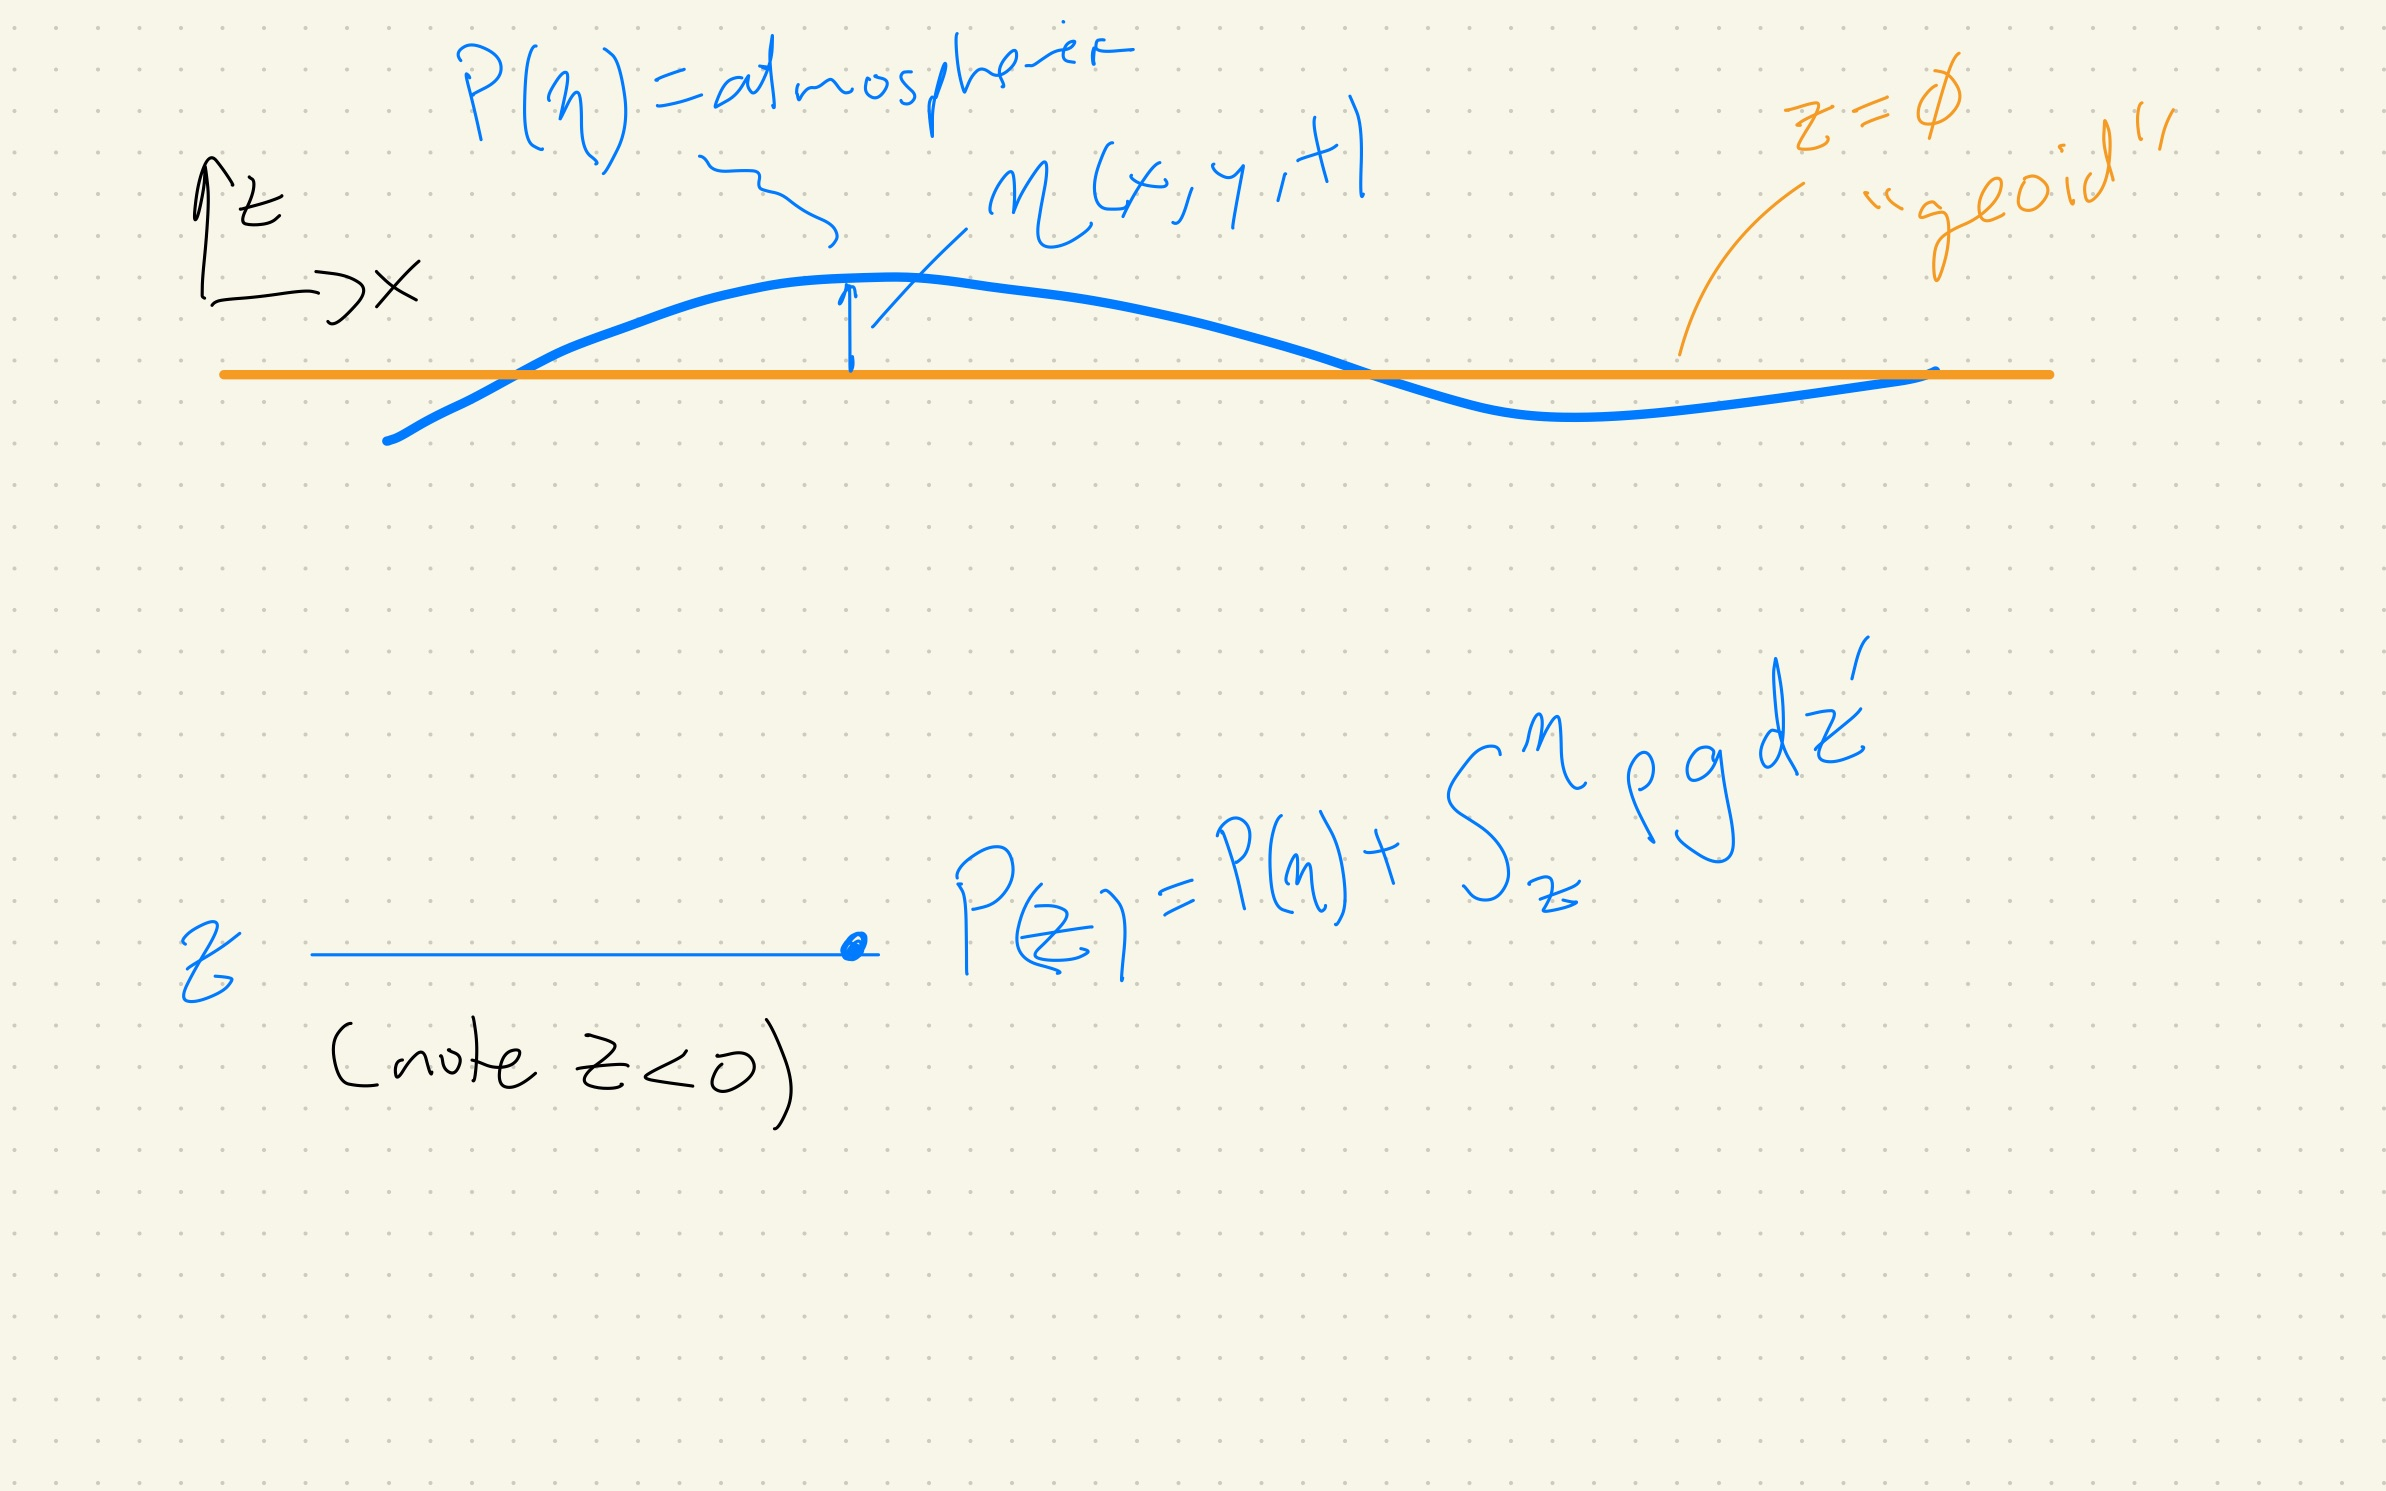
\includegraphics[keepaspectratio]{./imgs/S01_hydrostaticP.jpg}}
\caption{Hydrostatic approximation}
\end{figure}

Note that if the density is constant, then this simplifies to
\[ P(z) = P(\eta) + \rho g (\eta - z)\] and note that \(z<0\) so the
pressure increases as we go deeper.

The way to think about this is that the pressure at depth \(z\) is the
force per unit area needed to support the weight of the water above it,
which is the weight of the water column from \(z\) to the surface
\(\eta\).

Note that in the x- and y-momentum equations we have terms like
\[\frac{1}{\rho}\frac{\partial P}{\partial x}\] If the flow is
hydrostatic, then
\[\frac{Du}{Dt} = -\frac{1}{\rho}\frac{\partial P(\eta)}{\partial x} - \frac{1}{\rho}\frac{\partial}{\partial x} \int_z^{\eta} \rho g \, dz'\]
which we can use the Leibniz rule to write as
\[\frac{Du}{Dt} = -\frac{1}{\rho}\frac{\partial P(\eta)}{\partial x} - \frac{\partial \eta}{\partial x} g + \frac{1}{\rho}\int_z^\eta(x) \frac{\partial \rho}{\partial x} g\,\mathrm{d}z\]
For most practical purposes the first term is small because atmospheric
sea level pressure doesn't vary much, and does so over large areas. In
the third term, the contribution of the density gradient from
\(z=0 to \eta\) is small, so we simplify to:
\[\frac{Du}{Dt} = - \frac{\partial \eta}{\partial x} g - \frac{1}{\rho_0}\int_z^0 \frac{\partial \rho}{\partial x} g\,\mathrm{d}z\]
The first term on the right hand side is the acceleration due to sea
surface height gradients, and is called the \emph{barotropic pressure
gradient force}. The second term is the acceleration due to density
gradients, and is called the \emph{baroclinic pressure gradient force}.

\begin{figure}
\centering
\pandocbounded{\includegraphics[keepaspectratio]{./imgs/S01_baroclinicSketch.jpg}}
\caption{Baroclinic pressure gradient}
\end{figure}

As an example of the baroclinic pressure gradient force, in the above
sketch, the weight of the water at A is less than the weight of the
water column at B, so the pressure at A is less than the pressure at B,
and therefore there is a net pressure gradient from from B towards A,
and the water in the bottom layer will accelerate to the left. - soon
after there will be change in the surface pressure gradient as water
piles up at A and is removed from B. - note that we could
\emph{calculate} the pressure gradient force if we knew the thickness of
the upper layer \(h_1(x)\): -
\[-\frac{1}{\rho}\frac{\partial P}{\partial x} = g \frac{\rho_2-\rho_1}{\rho_2} \frac{\partial h_1}{\partial x}\]

\subsection{Application: Linear hydrostatic surface
waves}\label{application-linear-hydrostatic-surface-waves}

Consider a fluid with constant density \(\rho=\rho_0\), and lets ignore
the Coriolis force and viscosity. Ignoring the y-dimension, the
x-momentum equation is then:
\[ \frac{\partial u}{\partial t} + u\frac{\partial u}{\partial x} + w\frac{\partial u}{\partialz} = -\frac{1}{\rho_0}\frac{\partial P}{\partial x}\]
and the continuity equation is:
\[ \frac{\partial w}{\partial z} + \frac{\partial u}{\partial x} = 0\]
We can derive useful equations for surface waves if we assume that the
vertical accelerations are small compared to the gravity force so that
we can make the hydrostatic approximation, and that the waves are small
enough amplitude that the nonlinear terms can be ignored.

The x-momentum then becomes:
\[ \frac{\partial u}{\partial t} = -g\frac{\partial \eta}{\partial x}\]
We can simplify the continuity equation by integrating in depth and
assuming that \(\eta \ll H\) (the depth of the ocean):
\[ \int{-H}^{\eta} \frac{\partial u}{\partial x} \, dz \approx H \frac{\partial u}{\partial x}\]
The \(w\) term can also be integrated:
\[ \int{-H}^{\eta} \frac{\partial w}{\partial z} \, dz = w(\eta) - w(-H)\]
If the seafloor is flat then \(w(-H)=0\). \(w(\eta)\) is how fast the
sea surface is moving up and down, and can be written as
\[w(\eta) = \frac{\partial \eta}{\partial t} + \mathbf{u}\cdot\nabla\eta\]
but the linear assumption means that we can ignore the second term, so
\[w(\eta) = \frac{\partial \eta}{\partial t}\] so the continuity
equation becomes:
\[ H \frac{\partial u}{\partial x} + \frac{\partial \eta}{\partial t} = 0\]

\begin{figure}
\centering
\pandocbounded{\includesvg[keepaspectratio]{./imgs/S01_ContinuitySketch.svg}}
\caption{Continuity equation sketch}
\end{figure}

Hopefully this equation makes sense - if more water comes in from the
left than leaves to the right \(\partial u/\partial x <0\) and that
means that the sea surface must rise.

Combining these two equations yields a wave equation:
\[ \frac{\partial^2 \eta}{\partial t^2} = g H \frac{\partial^2 \eta}{\partial x^2}\]
This is a wave equation with wave phase speed \(c = \sqrt{gH}\), and
solutions of the form:
\[\eta = \eta_L \left(x+ct\right) + \eta_R \left(x-ct\right)\] where
\(\eta_L\) and \(\eta_R\) are the left and right moving waveforms set by
initial conditions.

Of course a very common case is that the wave is sinusoidal, so we can
write: \[\eta = \eta_0 \cos(k(x - c t) + \phi)\] which is a wave with
phase (peaks and troughs) propagating in the positive x-direction with
wavelength \(\lambda = 2\pi/k\) and wave speed \(c = \sqrt{gH}\).
\(\phi\) is an arbitrary phase that again could be set by initial
conditions. If we observe the wave at a fixed point then its angular
frequency will be \(\omega = ck = \sqrt{gH}k\). The direction of wave
propagation is given by the sign of \(k\) - if \(k>0\) then the wave is
propagating in the positive x-direction, and if \(k<0\) then it is
propagating in the negative x-direction.

\section{Viscous stress (shear
stress)}\label{viscous-stress-shear-stress}

Viscous stresses are related to pressure, in that they arise from
molecules hitting each other and transferring momentum. Viscous stress
is the portion of those stresses that are due to the relative motion of
the fluid. - Consider a fluid with two layers, one moving at speed \(U\)
and the other at speed \(0\). - There are no ``shear stresses'' inside
the layers because the molecules are, on average, moving with each
other. - The interface between the two layers has a shear stress as some
of the ``fast'' molecules hit the ``slow'' ones and transfer momentum
from the upper layer to the lower. - We use the notation \(\tau_{xz}\)
for this shear stress, where \(x\) is the direction of the flow and
\(z\) is the vertical direction, and the sign convention that
\(\tau_{xz}>0\) to mean that positive x-momentum is being transferred
\emph{downwards} (from the upper layer to the lower in this example).

\begin{figure}
\centering
\pandocbounded{\includesvg[keepaspectratio]{./imgs/S01_momentum_transfer.svg}}
\caption{Viscous stress sketch}
\end{figure}

Of course the same idea applies in all the directions (including the
x-direction), so the x-momentum equation has three shear stress terms
\(\tau_{xx}\), \(\tau_{xy}\), and \(\tau_{xz}\), which we will sometimes
write as \(\mathbf{\tau_x} = (\tau_{xx}, \tau_{xy}, \tau_{xz})\). -
These terms get used in the x-momentum equation by noting that on a
small cube, the shear stress can be exerted on the top face by the water
above, and is lost on the bottom face to the water below

\begin{figure}
\centering
\pandocbounded{\includesvg[keepaspectratio]{./imgs/S01_stress_xmom.svg}}
\caption{Sketch of stresses acting on a cube}
\end{figure}

\begin{itemize}
\tightlist
\item
  So the x-momentum equation becomes:
  \[\rho \delta x \delta y \delta z \frac{D u}{Dt} = \left(\tau_{xz}(x,y,z+\delta z) - \tau_{xz}(x,y,z)\right) \delta y \delta x + ...\]
  and as the cube is made infintesimally small, this becomes:
  \[\rho \frac{D u}{Dt} = \frac{\partial \tau_{xz}}{\partial z} + ...\]
\item
  including the oter directions yields:
  \[\rho \frac{D u}{Dt} = \frac{\partial \tau_{xx}}{\partial x} + \frac{\partial \tau_{xy}}{\partial y} + \frac{\partial \tau_{xz}}{\partial z} +  ...\]
\item
  or in vector notation:
  \[\rho \frac{D \mathbf{u}}{Dt} = \nabla \cdot \mathbf{\tau_x} + ...\]
  other momentum equations have the same terms and therefore there are
  \emph{nine} shear stress terms in total:
  \[\rho \frac{D v}{Dt} = \frac{\partial \tau_{yx}}{\partial x} + \frac{\partial \tau_{yy}}{\partial y} + \frac{\partial \tau_{yz}}{\partial z} + ...\]
  \[\rho \frac{D w}{Dt} = \frac{\partial \tau_{zx}}{\partial x} + \frac{\partial \tau_{zy}}{\partial y} + \frac{\partial \tau_{zz}}{\partial z} + ...\]
\end{itemize}

\subsubsection{Newtonian fluid shear
stresses}\label{newtonian-fluid-shear-stresses}

It is often useful to write the momentum equation using the shear
stresses, and we will do so in later classes. However, it is also useful
to assume the fluid is a \emph{Newtonian fluid}, which means that the
shear stresses are proportional to the velocity gradients:
\[\tau_{xz} = \mu \frac{\partial u}{\partial z}\] where \(\mu\) is the
\emph{dynamic viscosity} of the fluid (with units like kg/m/s). The
dynamic viscosity is a measure of how ``sticky'' the fluid is, and for
water it is about \(10^{-3} \mathrm{kg\,m^{-1}\,s^{-1}}\) at 20 deg C.
The shear stresses in the other directions are given by similar
equations: \[\tau_{xy} = \mu \frac{\partial u}{\partial y}\]
\[\tau_{xx} = \mu \frac{\partial u}{\partial x}\] or in vector form:
\[\mathbf{\tau_x} = \mu \nabla \mathbf{u}\]

Note that the momentum equation is almost always written in terms of the
\emph{kinematic viscosity} \(\nu = \mu/\rho\), which has units like
m\^{}2/s.

\begin{figure}
\centering
\pandocbounded{\includesvg[keepaspectratio]{./imgs/S01_stress_shear.svg}}
\caption{SKetch of shear stress in a Newtonian fluid}
\end{figure}

This means that the momentum equations become (including the pressure
gradient force):
\[\frac{D u}{Dt} = -\frac{1}{\rho}\frac{\partial P}{\partial x} + \nu \nabla^2 \mathbf{u} + ...\]
\[\frac{D v}{Dt} = -\frac{1}{\rho}\frac{\partial P}{\partial y} + \nu \nabla^2 \mathbf{v} + ...\]
\[\frac{D w}{Dt} = -\frac{1}{\rho}\frac{\partial P}{\partial z} - g + \nu \nabla^2 \mathbf{v} + ...\]
or in vector form:
\[\frac{D \mathbf{u}}{Dt} = -\frac{1}{\rho}\nabla P + \nu \nabla^2 \mathbf{u} - g\mathbf{k} + ...\]

\subsection{Summary}\label{summary}

So far we have derived - the conservation equations for a tracer \(C\),
where the concentration change at a fixed point changes in time due to
advection or diffusion/mixing. - The continuity equation for an
incompressible fluid, which says that the divergence of the velocity
field is zero. - The pressure gradient force and how it can readily be
evaluated from the seasurface height and density field to get the
barotropic and baroclinic pressure gradient forces respectively. -
Viscous stresses and how they can modify the flow due to velocity
gradients (shear). - This is basically all covered in FLuid Dynamics.
Next we will look at the Coriolis force and how it modifies the flow on
large time and space scales.
